\documentclass{article}
\usepackage[paperwidth=20.6cm,paperheight=9cm,margin=0cm,noheadfoot]{geometry}
\usepackage{amsmath,amssymb}
\usepackage{tikz}
\usetikzlibrary{arrows.meta,positioning,calc,backgrounds}
\usepackage{xcolor}
\usepackage[T1]{fontenc}
\usepackage{lmodern}
\usepackage{tgheros}
\usepackage{sansmath}          % sans-serif math
\renewcommand{\familydefault}{\sfdefault}
\sansmath                       % activate sans math globally
\pagestyle{empty}
\setlength{\parindent}{0pt}

% === Colors ===
\definecolor{deepblue}{HTML}{1A5276}
\definecolor{midblue}{HTML}{2980B9}
\definecolor{lightblue}{HTML}{AED6F1}
\definecolor{deeppurple}{HTML}{6C3483}
\definecolor{midpurple}{HTML}{8E44AD}
\definecolor{lightpurple}{HTML}{D2B4DE}
\definecolor{deeporange}{HTML}{B9470B}
\definecolor{midorange}{HTML}{E67E22}
\definecolor{lightorange}{HTML}{F5CBA7}
\definecolor{coralpink}{HTML}{E74C3C}
\definecolor{deepgray}{HTML}{2C3E50}
\definecolor{midgray}{HTML}{7F8C8D}
\definecolor{panelbg}{HTML}{FAFCFE}

\begin{document}
\vspace*{0pt}\noindent
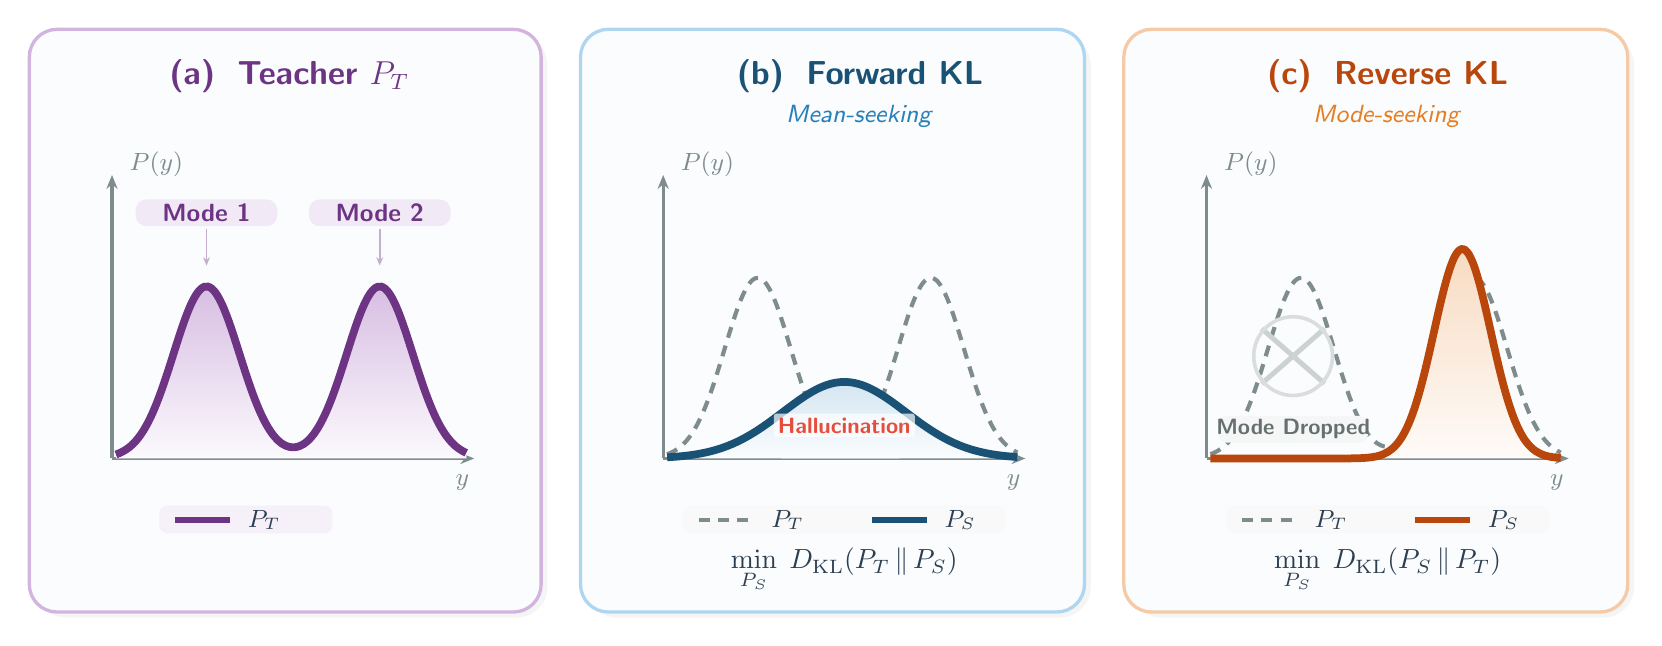
\begin{tikzpicture}[>=Stealth]

  % === Card dimensions ===
  % Each card: 6.0 wide, gap 0.5
  % card_a: x=0..6, card_b: x=6.5..12.5, card_c: x=13..19

  % =================== Panel (a): Teacher P_T ===================
  \fill[black, opacity=0.04, rounded corners=11pt] (0.08, -1.87) rectangle (6.58, 5.53);
  \fill[panelbg, rounded corners=10pt] (0, -1.8) rectangle (6.5, 5.6);
  \draw[lightpurple, line width=1.2pt, rounded corners=10pt] (0, -1.8) rectangle (6.5, 5.6);

  \begin{scope}[shift={(1.05, 0.15)}]
    \node[font=\large\bfseries, deeppurple] at (2.25, 4.85) {(a)\; Teacher $P_T$};
    
    % Axes
    \draw[-{Stealth[length=5pt,width=4pt]}, line width=1.2pt, midgray] 
      (0, 0) -- (4.6, 0);
    \node[font=\small, midgray, anchor=north] at (4.45, -0.08) {$y$};
    \draw[-{Stealth[length=5pt,width=4pt]}, line width=1.2pt, midgray] 
      (0, 0) -- (0, 3.6);
    \node[font=\small, midgray, anchor=south west] at (0.1, 3.45) {$P(y)$};
    
    % Fill
    \shade[top color=midpurple!35, bottom color=midpurple!3, smooth, samples=100, domain=0.05:4.5]
      plot (\x, {2.3*(exp(-((\x-1.2)^2)/(2*0.42^2)) + exp(-((\x-3.4)^2)/(2*0.42^2)))/(0.42*sqrt(2*pi))})
      -- (4.5,0) -- (0.05,0) -- cycle;
    
    % Curve
    \draw[deeppurple, line width=2.8pt, smooth, samples=100, domain=0.05:4.5]
      plot (\x, {2.3*(exp(-((\x-1.2)^2)/(2*0.42^2)) + exp(-((\x-3.4)^2)/(2*0.42^2)))/(0.42*sqrt(2*pi))});
    
    % Mode pills
    \fill[midpurple!12, rounded corners=4pt] (0.3, 2.95) rectangle (2.1, 3.29);
    \node[font=\small\bfseries, deeppurple] at (1.2, 3.12) {Mode 1};
    \fill[midpurple!12, rounded corners=4pt] (2.5, 2.95) rectangle (4.3, 3.29);
    \node[font=\small\bfseries, deeppurple] at (3.4, 3.12) {Mode 2};
    
    \draw[-{Stealth[length=3pt,width=2.5pt]}, deeppurple!40, line width=0.6pt] (1.2, 2.92) -- (1.2, 2.45);
    \draw[-{Stealth[length=3pt,width=2.5pt]}, deeppurple!40, line width=0.6pt] (3.4, 2.92) -- (3.4, 2.45);
    
    % Legend
    \fill[midpurple!8, rounded corners=3pt] (0.6, -0.6) rectangle (2.8, -0.95);
    \draw[deeppurple, line width=2.2pt] (0.8, -0.78) -- (1.5, -0.78);
    \node[font=\small, deepgray, anchor=west] at (1.6, -0.78) {$P_T$};
  \end{scope}

  % =================== Panel (b): Forward KL ===================
  \fill[black, opacity=0.04, rounded corners=11pt] (7.08, -1.87) rectangle (13.48, 5.53);
  \fill[panelbg, rounded corners=10pt] (7.0, -1.8) rectangle (13.4, 5.6);
  \draw[lightblue, line width=1.2pt, rounded corners=10pt] (7.0, -1.8) rectangle (13.4, 5.6);

  \begin{scope}[shift={(8.05, 0.15)}]
    \node[font=\large\bfseries, deepblue] at (2.5, 4.85) {(b)\; Forward KL};
    \node[font=\small, midblue] at (2.5, 4.35) {\textit{Mean-seeking}};
    
    % Axes
    \draw[-{Stealth[length=5pt,width=4pt]}, line width=1.2pt, midgray] 
      (0, 0) -- (4.6, 0);
    \node[font=\small, midgray, anchor=north] at (4.45, -0.08) {$y$};
    \draw[-{Stealth[length=5pt,width=4pt]}, line width=1.2pt, midgray] 
      (0, 0) -- (0, 3.6);
    \node[font=\small, midgray, anchor=south west] at (0.1, 3.45) {$P(y)$};
    
    % Hallucination zone
    \shade[top color=coralpink!22, bottom color=coralpink!2, smooth, samples=60, domain=1.5:3.0]
      plot (\x, {1.9*exp(-((\x-2.3)^2)/(2*0.78^2))/(0.78*sqrt(2*pi))})
      -- (3.0, 0) -- (1.5, 0) -- cycle;
    
    % Teacher — dashed
    \draw[midgray, line width=1.5pt, dash pattern=on 4pt off 3pt, smooth, samples=100, domain=0.05:4.5]
      plot (\x, {2.3*(exp(-((\x-1.2)^2)/(2*0.42^2)) + exp(-((\x-3.4)^2)/(2*0.42^2)))/(0.40*sqrt(2*pi))});
    
    % Student fill
    \shade[top color=midblue!20, bottom color=midblue!2, smooth, samples=100, domain=0.05:4.5]
      plot (\x, {1.9*exp(-((\x-2.3)^2)/(2*0.78^2))/(0.78*sqrt(2*pi))})
      -- (4.5,0) -- (0.05,0) -- cycle;
    
    % Student curve — ON TOP
    \draw[deepblue, line width=2.8pt, smooth, samples=100, domain=0.05:4.5]
      plot (\x, {1.9*exp(-((\x-2.3)^2)/(2*0.78^2))/(0.78*sqrt(2*pi))});
    
    % Hallucination label (no background, inside the zone)
    \node[font=\footnotesize\bfseries, coralpink, fill=white, fill opacity=0.7, text opacity=1, inner sep=1.5pt, rounded corners=1pt] at (2.3, 0.42) {Hallucination};
    
    % Legend
    \fill[midgray!5, rounded corners=3pt] (0.25, -0.6) rectangle (4.35, -0.95);
    \draw[midgray, line width=1.5pt, dash pattern=on 4pt off 3pt] (0.45, -0.78) -- (1.15, -0.78);
    \node[font=\small, deepgray, anchor=west] at (1.25, -0.78) {$P_T$};
    \draw[deepblue, line width=2.2pt] (2.65, -0.78) -- (3.35, -0.78);
    \node[font=\small, deepgray, anchor=west] at (3.45, -0.78) {$P_S$};
    
    % Formula
    \node[font=\normalsize, deepgray] at (2.3, -1.42) 
      {$\displaystyle\min_{P_S}\; D_{\mathrm{KL}}(P_T \,\|\, P_S)$};
  \end{scope}

  % =================== Panel (c): Reverse KL ===================
  \fill[black, opacity=0.04, rounded corners=11pt] (13.98, -1.87) rectangle (20.38, 5.53);
  \fill[panelbg, rounded corners=10pt] (13.9, -1.8) rectangle (20.3, 5.6);
  \draw[lightorange, line width=1.2pt, rounded corners=10pt] (13.9, -1.8) rectangle (20.3, 5.6);

  \begin{scope}[shift={(14.95, 0.15)}]
    \node[font=\large\bfseries, deeporange] at (2.3, 4.85) {(c)\; Reverse KL};
    \node[font=\small, midorange] at (2.3, 4.35) {\textit{Mode-seeking}};
    
    % Axes
    \draw[-{Stealth[length=5pt,width=4pt]}, line width=1.2pt, midgray] 
      (0, 0) -- (4.6, 0);
    \node[font=\small, midgray, anchor=north] at (4.45, -0.08) {$y$};
    \draw[-{Stealth[length=5pt,width=4pt]}, line width=1.2pt, midgray] 
      (0, 0) -- (0, 3.6);
    \node[font=\small, midgray, anchor=south west] at (0.1, 3.45) {$P(y)$};
    
    % Teacher — dashed
    \draw[midgray, line width=1.5pt, dash pattern=on 4pt off 3pt, smooth, samples=100, domain=0.05:4.5]
      plot (\x, {2.3*(exp(-((\x-1.2)^2)/(2*0.42^2)) + exp(-((\x-3.4)^2)/(2*0.42^2)))/(0.40*sqrt(2*pi))});
    
    % Student fill
    \shade[top color=midorange!28, bottom color=midorange!3, smooth, samples=100, domain=0.05:4.5]
      plot (\x, {2.4*exp(-((\x-3.25)^2)/(2*0.36^2))/(0.36*sqrt(2*pi))})
      -- (4.5,0) -- (0.05,0) -- cycle;
    
    % Student curve — ON TOP
    \draw[deeporange, line width=2.8pt, smooth, samples=100, domain=0.05:4.5]
      plot (\x, {2.4*exp(-((\x-3.25)^2)/(2*0.36^2))/(0.36*sqrt(2*pi))});
    
    % Mode dropped X
    \draw[midgray!40, line width=1.8pt] (0.7, 0.95) -- (1.5, 1.65);
    \draw[midgray!40, line width=1.8pt] (0.7, 1.65) -- (1.5, 0.95);
    \draw[midgray!30, line width=1.3pt] (1.1, 1.3) circle (0.5);
    
    \fill[midgray!8, rounded corners=3pt] (0.15, 0.2) rectangle (2.05, 0.54);
    \node[font=\footnotesize\bfseries, midgray!80!black] at (1.1, 0.37) {Mode Dropped};
    
    % Legend
    \fill[midgray!5, rounded corners=3pt] (0.25, -0.6) rectangle (4.35, -0.95);
    \draw[midgray, line width=1.5pt, dash pattern=on 4pt off 3pt] (0.45, -0.78) -- (1.15, -0.78);
    \node[font=\small, deepgray, anchor=west] at (1.25, -0.78) {$P_T$};
    \draw[deeporange, line width=2.2pt] (2.65, -0.78) -- (3.35, -0.78);
    \node[font=\small, deepgray, anchor=west] at (3.45, -0.78) {$P_S$};
    
    % Formula
    \node[font=\normalsize, deepgray] at (2.3, -1.42) 
      {$\displaystyle\min_{P_S}\; D_{\mathrm{KL}}(P_S \,\|\, P_T)$};
  \end{scope}

\end{tikzpicture}
\end{document}
